\documentclass[12pt,fleqn]{article}\usepackage{../../common}
\begin{document}
Yükseklik Fonksiyonu (Tepeler) Arasından En Düz, Optimal Yürüyüş Yolunu Bulmak

Elimizde bir alan içindeki yükseklikleri veren bir fonksiyon $f(x,y)$
olduğunu düşünelim. Acaba verili bir başlangıç ve bitiş noktası arasındaki
en ``rahat'' gidiş yolunu nasıl buluruz? 

Yükseklikler bir $E(x,y)$ fonksiyonunda olsun. Yolları nasıl temsil ederiz?
Bir parametrik eğri kullanabiliriz, mesela 

$$
x(t) = a_0 + a_1 t + a_2 t^2 + a_3 t^3 + a_4 t^4
$$

$$
y(t) = b_0 + b_1 t + b_2 t^2 + b_3 t^3 + b_4 t^4
$$

İstediğimiz derecede polinom parametrize eğrileri nasıl yaratacağımızı
biliyoruz [3]. Böylece doğru, optimal bir yolu bulmak demek
$a_0,a_1,a_2,a_3,b_0,b_1,b_2,b_3$ katsayılarını doğru bulmak demek
olacaktır. Bir optimizasyon problemi yani.

Peki o zaman optimize, minimize edilecek bedel fonksiyonu ne olmalı? Burada
farklı yaklaşımlar olabilir. Kimisi eğri altına düşen yüksekliklerin
toplamını bir çizgi entegrali ile hesaplamak isteyebilir. Fakat bu yaklaşım
yüksekliklerden genel olarak uzak dursa da mesela çok inişli çıkışlı
yolları hala tercih eder, ama bu tür yolların yürüyüş olarak yorucu
olacağını biliyoruz. 1000 metrelik bir tepeye çıkıp onun üzerinde düz
yürümek habire 1000 metreyi inmek çıkmaktan çok daha rahat.

Şu şekilde bir bedel belki daha iyi; Bir eğriyi düşünelim, onun $z$
eksenindeki yansıması da bir eğridir, $x,y$ düzlemindeki yansıması bir
başka eğri. Bu eğrilerin {\em uzunluğunu} hesaplarsak [2] ve dikey yöndeki
uzunluğu yatay olan uzunluğu farklı ağırlıklarla çarpıp toplarsak bu bir
bedeli temsil eder. Ağırlık dikey/yatay uzunluklar için 5/1 oranında
olabilir, o zaman yatay yöndeki bir uzunluk / katedilen yol dikeye göre 5
kat daha tercih edilir olur.

Önce yükseklikleri ve eğrileri iki örnek üzerinde görelim. Bir rasgele
tepe, ve bir rasgele yol çiziyoruz,

\begin{minted}[fontsize=\footnotesize]{python}
from mpl_toolkits.mplot3d import Axes3D
from scipy.spatial.distance import cdist
from matplotlib import cm

def gfunc1(x, y):
    s1 = 2.2; x1 = 2.0; y1 = 2.0
    g1 = np.exp( -4 *np.log(2) * ((x-x1)**2+(y-y1)**2) / s1**2)
    return g1 * 10.0

def plot_surf_path(myfunc,a0,a1,a2,a3,a4,b0,b1,b2,b3,b4):

    D = 50
    x = np.linspace(0,5,D)
    y = np.linspace(0,5,D)
    xx,yy = np.meshgrid(x,y)
    zz = myfunc(xx,yy)

    fig = plt.figure()
    ax = fig.gca(projection='3d')
    ax.set_xlim(0,5)
    ax.set_ylim(0,5)
    surf = ax.plot_wireframe(xx, yy, zz,rstride=10, cstride=10)

    t = np.linspace(0,1.0,100)

    x = a0 + a1*t + a2*t**2 + a3*t**3 + a4*t**4 
    y = b0 + b1*t + b2*t**2 + b3*t**3 + b4*t**4

    ax.plot3D(x, y, gfunc1(x,y),'r.')
\end{minted}

\begin{minted}[fontsize=\footnotesize]{python}
# 1. gidis yolunun tanimi, uzun yoldan dolanarak gidiyor
a1,a2,a3 = 1.5, 8.1, 4.0
b1,b2,b3 = 0.3, 0.4, 23.3
a0,b0=(1.0,1.0)
ex,ey=(0.3,4.0)
a4 = ex - a0 - (a1+a2+a3)
b4 = ey - b0 - (b1+b2+b3)
test_coefs1 = (a0,a1,a2,a3,a4,b0,b1,b2,b3,b4)
plot_surf_path(gfunc1,a0,a1,a2,a3,a4,b0,b1,b2,b3,b4)

plt.savefig('calc_multi_40_elev_01.png')
\end{minted}

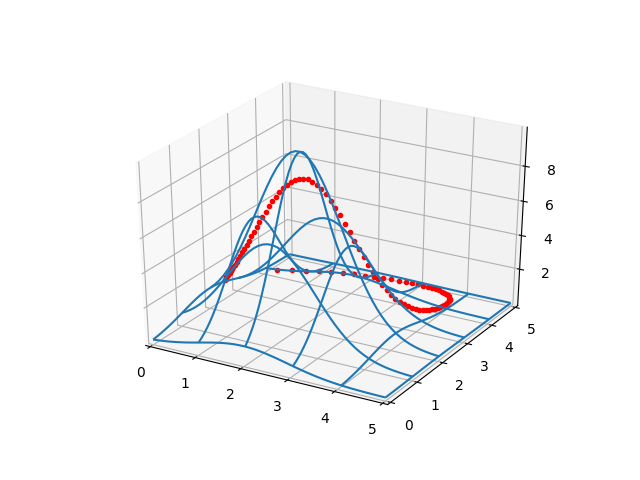
\includegraphics[width=20em]{calc_multi_40_elev_01.png}

Başlangıç ve bitiş noktalarını nasıl formüle dahil ettiğimize dikkat, $t=0$
olduğu anda $x(t),y(t)$ değerleri sırasıyla $a_0$ ve $b_0$'dir bunlar başlangıç
değerleridir. Bitiş noktası ise $t=1$ anında sahip olunması gereken değerdir,
bu noktada

$$
x(1) = a_0 + a_1 + a_2 + a_3 + a_4 ,\quad
y(1) = b_0 + b_1 + b_2 + b_3 + b_4 
$$

olacağı için bitiş noktalarına $e_x,e_y$ diyelim, $x(t)$ için $a_1,a_2,a_3$
katsayılarının değişmesine izin veririz, fakat sonuncu katsayı $a_4$'un ne
olacağını formülde $e_x$ üzerinden zorlarız, yani $a_4 = e_x - (a_0 + a_1 + a_2
+ a_3)$ hesabını yaparız. Böylece $a_0 + a_1 + a_2 + a_3 + a_4$ toplamı
$e_x$ sonucunu vermelidir. $y(t)$ ve $e_y$ için benzer mantığı kullanırız.

Eğer üstteki gidiş yoluna kuşbakışı, iki boyutlu ortamda bakmak istersek,

\begin{minted}[fontsize=\footnotesize]{python}
t = np.linspace(0,1.0,100)
x = a0 + a1*t + a2*t**2 + a3*t**3 + a4*t**4 
y = b0 + b1*t + b2*t**2 + b3*t**3 + b4*t**4
plt.xlim(0,5.0)
plt.ylim(0,5.0)
plt.plot(x,y)
plt.savefig('calc_multi_40_elev_02.png')
\end{minted}

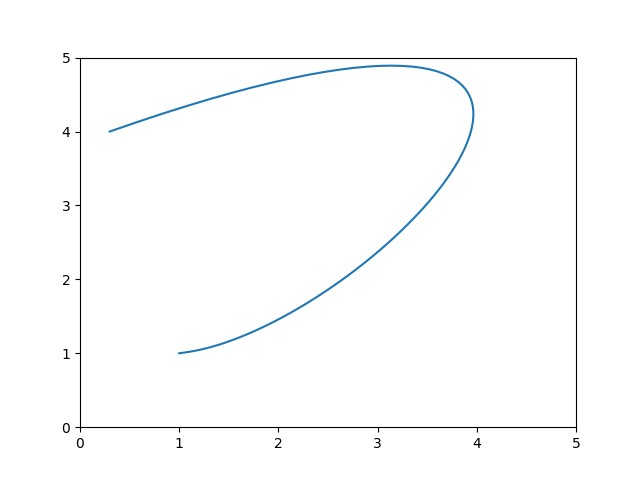
\includegraphics[width=20em]{calc_multi_40_elev_02.png}

Bu biraz önce bahsettiğimiz yatay düzlemdeki yansıma.

Şimdi ikinci bir gidiş yoluna bakalım, başlangıç noktası aynı ama bitiş farklı,

\begin{minted}[fontsize=\footnotesize]{python}
# 2. gidis yolunun tanimi, dik cikip iniyor
a1,a2,a3 = 1.5, 3.0, 1.0
b1,b2,b3 = 0.0, 1.0, 1.0
a0,b0=(1.0,1.0)
ex,ey=(0.3,4.0)
a4 = ex - a0 - (a1+a2+a3)
b4 = ey - b0 - (b1+b2+b3)
test_coefs2 = (a0,a1,a2,a3,a4,b0,b1,b2,b3,b4)
plot_surf_path(gfunc1,a0,a1,a2,a3,a4,b0,b1,b2,b3,b4)
plt.savefig('calc_multi_40_elev_03.png')
\end{minted}

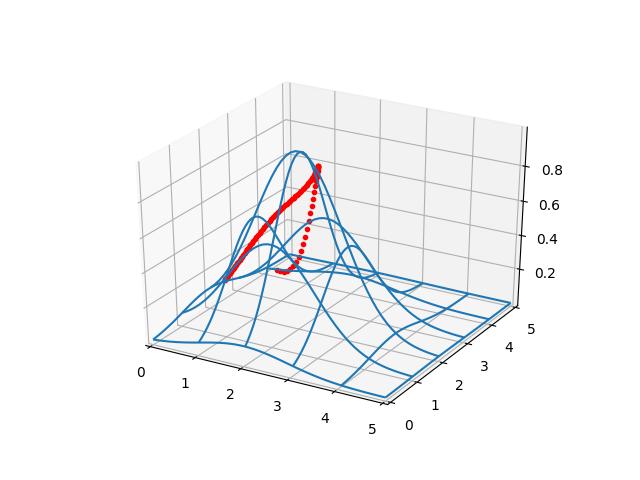
\includegraphics[width=20em]{calc_multi_40_elev_03.png}

Bu yolları tabii ki rasgele parametreler üzerinden yarattık, bunlar optimal
yollar değiller.

$$
\int_{t=0}^{t=1} f(x(t),y(t)) \sqrt {x'(t)^2 + y'(t)^2} \ud t
$$


\begin{minted}[fontsize=\footnotesize]{python}
import sympy

vars = 't a0 a1 a2 a3 a4 b0 b1 b2 b3 b4 gamma x y'
t, a0, a1, a2, a3, a4, b0, b1, b2, b3, b4, gamma, x, y = sympy.symbols(vars)

xdef = a0 + a1*t + a2*t**2 + a3*t**3 + a4*t**4
ydef = b0 + b1*t + b2*t**2 + b3*t**3 + b4*t**4

dxdt = sympy.diff(xdef,t)
print (dxdt)
dydt = sympy.diff(ydef,t)
print (dydt)
sqrtdef = sympy.sqrt(sympy.diff(xdef,t)**2 + sympy.diff(ydef,t))
print (sqrtdef)
\end{minted}

\begin{verbatim}
a1 + 2*a2*t + 3*a3*t**2 + 4*a4*t**3
b1 + 2*b2*t + 3*b3*t**2 + 4*b4*t**3
sqrt(b1 + 2*b2*t + 3*b3*t**2 + 4*b4*t**3 + (a1 + 2*a2*t + 3*a3*t**2 + 4*a4*t**3)**2)
\end{verbatim}

\begin{minted}[fontsize=\footnotesize]{python}
sqrdef = sympy.diff(xdef,t)**2 + sympy.diff(ydef,t)
\end{minted}

\begin{minted}[fontsize=\footnotesize]{python}
xsubs = {a0: 2, a1: 2, a2: 2, a3: 2, a4: 2, t:0.5}
xval = xdef.subs(xsubs)
ysubs = {b0: 3, b1: 3, b2: 3, b3: 3, b4: 3, t:0.5}
yval = ydef.subs(ysubs)
sqrval = sqrtdef.subs(xsubs).subs(ysubs)
g1 = gfunc1(float(xval),float(yval))
print (xval, yval, sqrval, g1)
\end{minted}

\begin{verbatim}
3.87500000000000 5.81250000000000 7.21110255092798 0.00032302357084224476
\end{verbatim}

\begin{minted}[fontsize=\footnotesize]{python}
pa0,pb0=(1.0,1.0)
pex,pey=(0.3,4.0)
ts = np.linspace(0,1,20)
def calcint_g1(pars):
    pa1,pa2,pa3,pb1,pb2,pb3=pars
    pa4 = pex - pa0 - (pa1+pa2+pa3)
    pb4 = pey - pb0 - (pb1+pb2+pb3)
    argsubs = {a1:pa1, a2:pa2, a3:pa3, a4:pa4, \
               b1:pb1, b2:pb2, b3:pb3, b4:pb4}
    ys = []
    for tcurr in ts:
       sqrval = sqrdef.subs(argsubs).subs({t:tcurr})
       if sqrval < 0: sqrval = 0    
       xval = xdef.subs(argsubs).subs({a0: pa0}).subs({t:tcurr})
       yval = ydef.subs(argsubs).subs({b0: pb0}).subs({t:tcurr})
       prod1 = gfunc1(float(xval),float(yval))*sqrval
       ys.append(prod1)
    W = np.trapz(ys,x=ts)
    return W
\end{minted}


\begin{minted}[fontsize=\footnotesize]{python}
from scipy.optimize import minimize, Bounds, SR1, BFGS

LIM = 5.0
pa1,pa2,pa3 = 0,0,0
pb1,pb2,pb3 = 0,0,0
x0 = pa1,pa2,pa3,pb1,pb2,pb3
opts = {'maxiter': 20, 'verbose': 0}
res = minimize (fun=calcint_g1,x0=x0,
                method='trust-constr',
                hess = BFGS (),
                bounds=Bounds([-LIM, -LIM, -LIM, -LIM, -LIM, -LIM],
                              [LIM, LIM, LIM, LIM, LIM, LIM]),
                options=opts)
print (res['x'])
\end{minted}

\begin{verbatim}
[-0.35628684 -2.58099677 -3.26315201 -3.87505375  1.12278098  1.70215256]
\end{verbatim}

\begin{minted}[fontsize=\footnotesize]{python}
a1,a2,a3,b1,b2,b3 = list(res['x'])
a4 = ex - pa0 - (a1+a2+a3)
b4 = ey - pb0 - (b1+b2+b3)
test_coefs1 = (pa0,a1,a2,a3,a4,pb0,b1,b2,b3,b4)
plot_surf_path(gfunc1,pa0,a1,a2,a3,a4,pb0,b1,b2,b3,b4)
plt.savefig('calc_multi_40_elev_07.jpg')
\end{minted}

\begin{minted}[fontsize=\footnotesize]{python}
def gfunc2(x, y):
    s1 = 2.2; x1 = 2.0; y1 = 2.0
    g1 = np.exp( -4 *np.log(2) * ((x-x1)**2+(y-y1)**2) / s1**2)
    s2 = 1.2; x2 = 4.0; y2 = 1.0
    g2 = np.exp( -4 *np.log(2) * ((x-x2)**2+(y-y2)**2) / s2**2)
    return g1*10.0 + g2*10.0
\end{minted}


\begin{minted}[fontsize=\footnotesize]{python}
# sort of optimal
a1,a2,a3,b1,b2,b3  = 0.10273294,  0.07639032, -0.02498681, -0.0396142,  -0.00716718, -0.14862271
a4 = ex - pa0 - (a1+a2+a3)
b4 = ey - pb0 - (b1+b2+b3)
test_coefs2 = (pa0,a1,a2,a3,a4,pb0,b1,b2,b3,b4)
plot_surf_path(gfunc2,pa0,a1,a2,a3,a4,pb0,b1,b2,b3,b4)
plt.savefig('calc_multi_40_elev_08.jpg')
\end{minted}






[devam edecek]

Kaynaklar 

[1] Bayramlı, Sayısal Bilim, {\em Sayısal Entegrasyon (Numerical Integration)}

[2] Bayramlı, Çok Boyutlu Calculus, {\em Ders 6, Eğri Uzunluğu}

[3] Bayramlı, Çok Boyutlu Calculus, {\em Ders 5, İki Nokta Arasında Parametrize Edilmiş Eğri}

[5] Bayramlı, Fonksiyonel Analiz ve Optimizasyon, {\em Newton-umsu Metotlar, DFP, BFGS }

\end{document}

